%%%%%%%%%%%%%%%%%%%%%%%%%%%%%%%%%%%%% 
%% LE2I beamer template
%% Guillaume Lemaitre, October 2014
%%%%%%%%%%%%%%%%%%%%%%%%%%%%%%%%%%%%% 

\documentclass{beamer}

\usepackage[utf8]{inputenc}
\usepackage[T1]{fontenc} 
\usetheme{le2i} 

%% The amssymb package provides various useful mathematical symbols
\usepackage{amssymb}
%% The amsthm package provides extended theorem environments
\usepackage{amsthm}

%% amsmath for math environment
\usepackage{amsmath}

\DeclareMathOperator*{\argmin}{arg\,min}
\DeclareMathOperator*{\argmax}{arg\,max}
\DeclareMathOperator*{\sign}{sign}

%% figure package
\usepackage{epsf,graphicx}
\usepackage{epstopdf}
\usepackage{subfigure}
\usepackage{transparent}
\usepackage{algorithmicx}
\usepackage{algpseudocode}
%\usepackage{algorithm2e}

%% In order to draw some graphs
\usepackage{tikz,xifthen}
\usepackage{tikz-qtree}
\usepackage{adjustbox}
\usetikzlibrary{decorations.pathmorphing}
\usetikzlibrary{fit}
\usetikzlibrary{backgrounds}
\usetikzlibrary{shapes,arrows,shadows}
\usetikzlibrary{calc,decorations.pathreplacing,decorations.markings,positioning}
\usetikzlibrary{snakes,decorations.text,shapes,patterns}
% \usepackage{scalefnt,lmodern,booktabs}

%% Package for cross and tick symbols
\usepackage{pifont}
\newcommand{\tick}{\color{green!60!black!80}\ding{51}}
\newcommand{\cross}{\color{red!60!black!80}\ding{55}}

\title{Segmentation}
\author{Guillaume Lemaitre}
%\date{Define the event \\ day\textsuperscript{th} Month Year}

\institute{Universit\'e de Bourgogne} 

%% Uncomment if you want to avoid thousand of bullet inside the menu
% \usepackage{etoolbox}
% \makeatletter
% \patchcmd{\slideentry}{\advance\beamer@xpos by1\relax}{}{}{}
% \def\beamer@subsectionentry#1#2#3#4#5{\advance\beamer@xpos by1\relax}%
% \makeatother

\begin{document}

% Show the title page
\begin{frame}
  \titlepage
\end{frame}

% Show the table of contents
\begin{frame}
  \tableofcontents[sectionstyle=show,subsectionstyle=show,subsubsectionstyle=hide]
\end{frame}

%---------------
\section{Introduction}
\begin{frame}
\frametitle{Image Segmentation}
\begin{itemize}
\item Image segmentation is the partition of the image into non-overlapping regions, where their union is an entire image
\item Purpose of segmentation: decompose an image into meaningful parts with respect to unique application
\item Segmentation is based on the information taken from the image such as greylevel, texture, color and depth or motion
\end{itemize}
\end{frame}

\begin{frame}
\frametitle{Image Segmentation}
\begin{block}{Applications ...}
\begin{itemize}
\item Identifying objects in a scene for object-based measurements/recognition
\item Identifying objects in a moving scene for object based video compression
\item Identifying objects at different depths
\item Its a necessary and fundamental step in a general frameworks of detection, tracking or classification 
\end{itemize}
\end{block}
\end{frame}

\begin{frame}
\frametitle{Image Segmentation}
\begin{block}{Techniques}
\begin{itemize}
\item Region-based
\begin{itemize}
\item Region growing
\item Split and merge
\end{itemize}
\item Edge-based 
\begin{itemize}
\item Contours/ boundary surface 
\item Deformable wrapping
\item Deformable registration to atlases
\end{itemize}
\item Clustering-based 
\begin{itemize}
\item Threshold
\item K-means
\item Hierarchical clustering, Graph cuts 
\end{itemize}
\item Texture-based
\end{itemize}
\end{block}
\end{frame}
%---------------
\begin{frame}
\frametitle{Image Segmentation}
\begin{center}
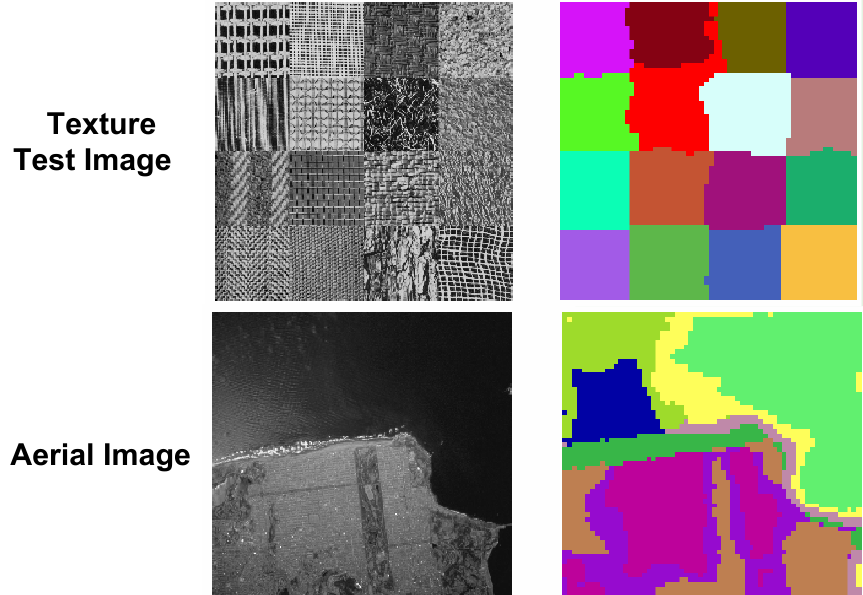
\includegraphics[scale=0.35]{images/L8_TextureAerial.png}
\end{center}
\end{frame}
%-------------
\section{Region Based}
%--------------
\begin{frame}
\frametitle{Region Based Segmentation}
\begin{block}{Region Growing}
\begin{itemize}
\footnotesize{
\item Starting with some pixels (seeds) representing distinct image regions
\item Grow the region of each seed, using connected pixels until they cover the entire image
\item Two rules: growth mechanism and region homogeneity after each growth step
\item {\color{blue}Growth mechanism: for each stage $k$ and each region $R_{i}(k), i= 1,..., N$, check if there are unclassified pixels in 8 neighborhood of each pixel in the region}
\item Region homogeneity: Pixel $P_{x,y}$ can join $R_{i}(k)$ if $\vert f(x,y) - \mu_{R_{i}(k)} \vert \leq  \Delta $ 
}
\end{itemize}
\end{block}
\end{frame}

\begin{frame}
\frametitle{Region Based Segmentation}
\begin{block}{Region Growing}
\begin{itemize}
\item Merging two region: 
\item Mean ($\mu$) and standard deviation ($\sigma$) of each region ($R_{i}$) can be used to decide if two region can merge: 
$$ \mu_{R_{i}} = \frac{1}{n}\sum\limits_{(r,c)\in R_{i}} I(r,c) $$ 
$$ \sigma_{R_{i}} = \sqrt{\frac{1}{n}\sum\limits_{(r,c) \in R_{i}} [I(r,c) - M_{R_{i}}]^{2}}$$ 
$$\text{if     } \vert M_{R_{1} - M_{R_{2}}} \vert < k \sigma_{R_{i}}  \text{  for  } i= 1,2  \text{  two region are merged} $$ 
\end{itemize}

\end{block}
\end{frame}

\begin{frame}
\frametitle{Image Segmentation}
\framesubtitle{Region Based Methods}
\begin{block}{Region Growing - Kind of unseeded RG}
Using one seed only, the first pixel: \\
\scriptsize{
\begin{algorithmic}
 \For{All the pixels n the image}
 \If{$P_{x,y} \notin R_{1,2,....,n}$}
 	\State $P_{x,y} \in R_{n+1}$
 	\For{S: The 4 or 8 neighbors of $x,y$}
 		\If{$P_{x',y'}  \notin R_{1,2,...,n}$}
 			\If{$\vert f(x',y') - \mu_{R_{i}} \vert \leq  \Delta $}
 				\State $P_{x',y'} \in R_{n+1}$
 				\State Search the neighbors of $x',y'$ 
 			\Else
 				\State $P_{x',y'} \in R_{n+2}$
 				\State Search the 4 or 8 neighbors of $x',y'$
 			\EndIf
 		\EndIf
 	\EndFor
 \EndIf
 \EndFor
 \end{algorithmic}
}
\end{block}
\end{frame}

\begin{frame}
\frametitle{Region Based Segmentation}
\begin{block}{Region Growing}
\centering{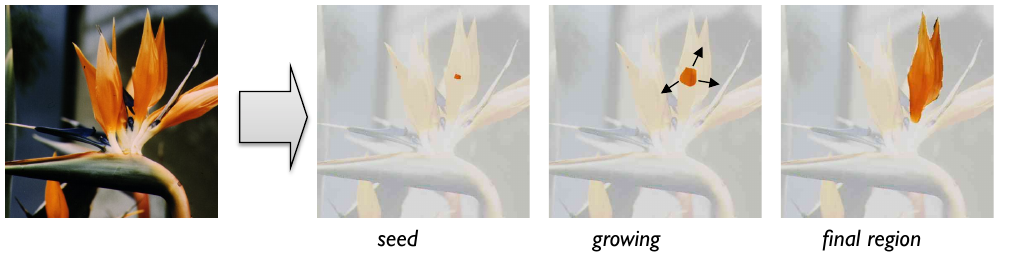
\includegraphics[scale=0.4]{images/L8_ex_RG.png}}
\end{block}
{\color{red} Fabrice example}
\end{frame}

%-------------
\begin{frame}
\frametitle{Region Based Segmentation}
\begin{block}{Split Method}
\begin{itemize}
\footnotesize{
\item Opposite of previous method 
\item Top to down approach
\item Starts with the assumption that the whole image is a homogeneous region
\item If this is not true, subdivides the image to smaller homogeneous regions 
\item If original Image $I_{N \times N} = I_{2^n \times 2^n}$ $\rightarrow$ square produced regions $R^{i}_{M \times M} = R^{i}_{2^m \times 2^m}$ 
\item Recursive procedure $\Rightarrow$ Image representation can be modeled by a tree whose nodes have four sons each
\item \textbf{Quadtree} 
\item {\color{red} Created regions might be adjacent and homogeneous but are not merged}}
\end{itemize}
\end{block}
\end{frame}

\begin{frame}
\frametitle{Region Based Segmentation}
\begin{block}{Split Method}
\scriptsize{Criterion of Homogeneity: Variance}
\begin{center}
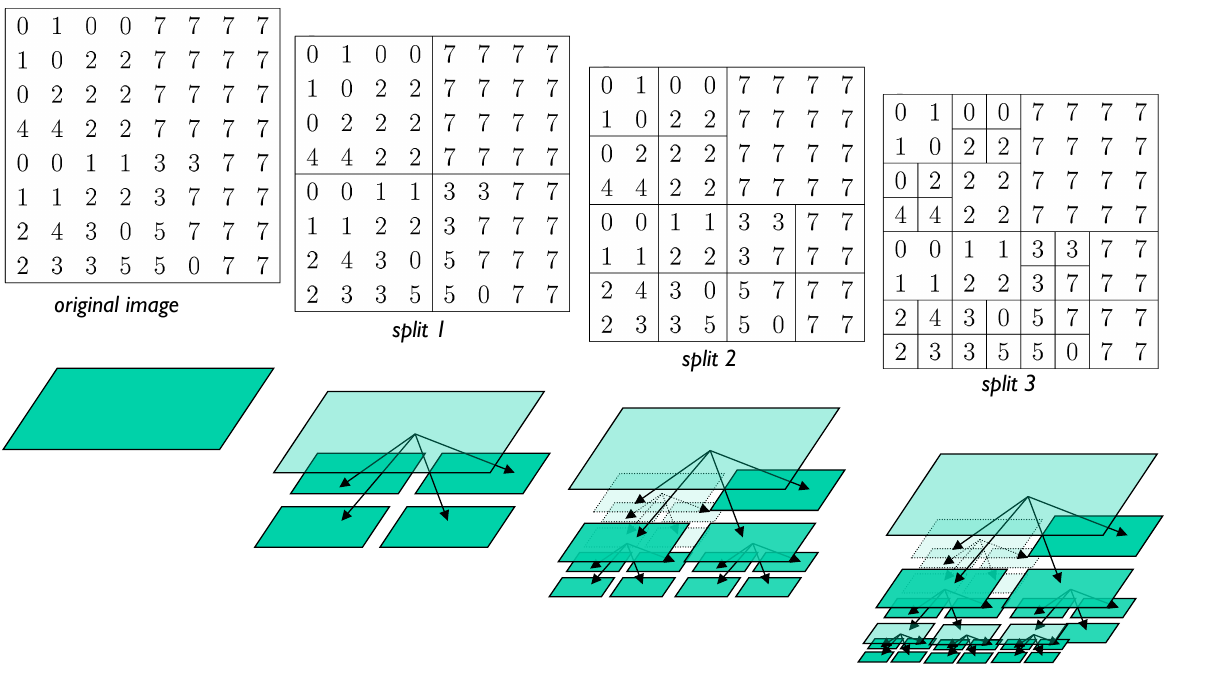
\includegraphics[scale=0.3]{images/L8_Split3.png}
\end{center}
\end{block}
\end{frame}

\begin{frame}
\frametitle{Region Based Segmentation}
\begin{block}{Split and Merge Method}
\begin{itemize}
\item Iterative technique that included both splitting and merging at each iteration
\item If $R_{i}$ is inhomogeneous, split $R_{i}$ into four sub-regions
\item If two adjacent region $R_{i}$ and $R_{j}$ are homogeneous, merge them 
\item The algorithm stops when no more merge or split is possible 
\item {\color{green} Produce more compact regions than just splitting}
\end{itemize}
\end{block}
\end{frame}

\begin{frame}
\frametitle{Region Based Segmentation}
\begin{block}{Split and Merge Method - Data Structure}
\begin{columns}
\column{0.38\textwidth}
\begin{itemize}
\item \footnotesize{Quadtree for splitting}\\
\scriptsize{Top-down approach, regions are split but not merged}
\item \footnotesize{RAG(region adjacency graph)}\\
\scriptsize{Split and merge iteratively at each iteration of quadtree partitioning\\
RAG has quadtree embedded that represent 4 relations\\
4 adjacent relations(one per square side)}
\end{itemize}
\column{0.7\textwidth}
\centering{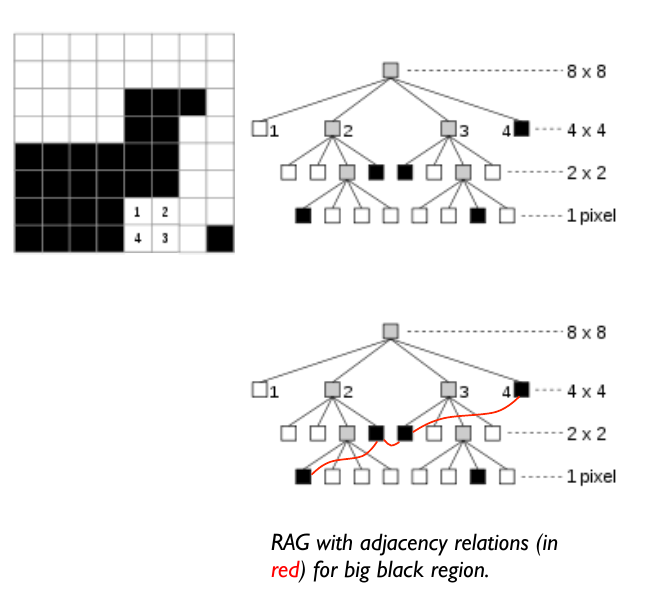
\includegraphics[scale=0.37]{images/L8_SplitMerge4.png}}
\end{columns}
\end{block}
\end{frame}
%--------------
% Examples
\begin{frame}
\frametitle{Region Based Segmentation}
\begin{block}{Region Growing}
\centering{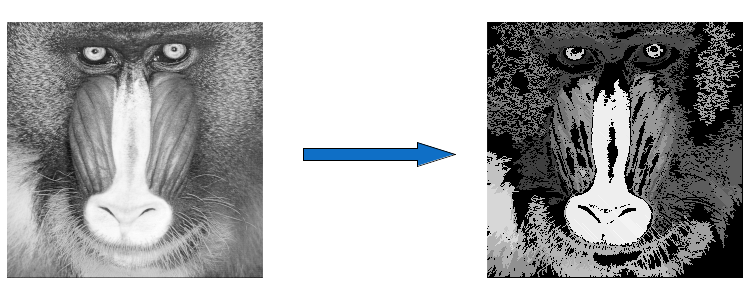
\includegraphics[scale=0.24]{images/L8_ex_RG2.png}}
\end{block}

\begin{block}{Split and Merge}
\centering{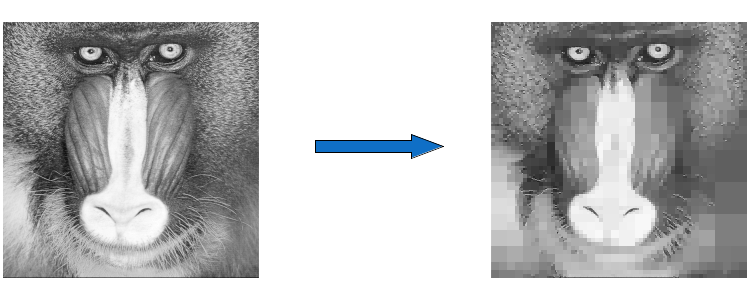
\includegraphics[scale=0.24]{images/L8_ex_SM2.png}}
\end{block}
\end{frame}

\begin{frame}
\frametitle{Region Based Segmentation}
\begin{block}{Splitting}
\centering{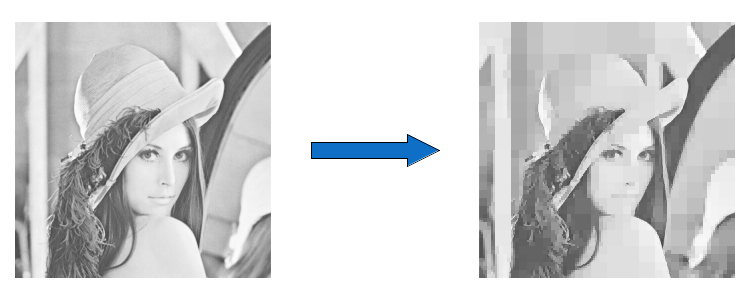
\includegraphics[scale=0.24]{images/L8_ex_S.png}}
\end{block}

\begin{block}{Split and Merge}
\centering{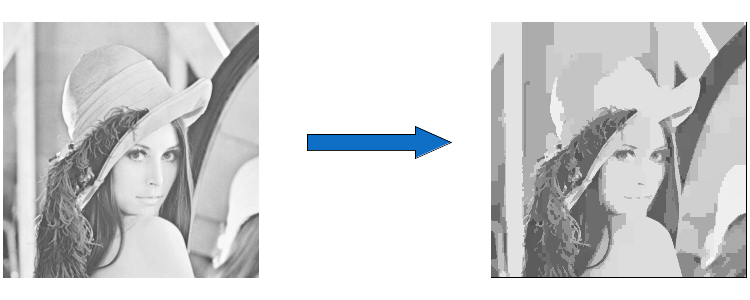
\includegraphics[scale=0.24]{images/L8_ex_SM.png}}
\end{block}
\end{frame}

%-----------------------------
\section{Clustering Based}

\begin{frame}
\frametitle{Clustering}
\begin{block}{Image Clustering vs. Image Segmentation}
\begin{itemize}
\item In clustering the grouping is done in measurement space
\item In segmentation the grouping is done in spatial domain
\end{itemize}
\end{block}

\begin{block}{Approaches}
\begin{itemize}
\item Threshold
\item K-means
\item Hierarchical clustering, Graph cut, ...
\end{itemize}
\end{block}
\end{frame}

\begin{frame}
\frametitle{Clustering}
\footnotesize{
\begin{itemize}
\item Grouping of pixels considering 1 or more features
\item Grouping similar features, feature selection
\item Spatial distribution of the pixels is not considered 
\item Feature space is considered
\item Clusters has compact shape, spherical, ellipsoidal, elongated, .. 
\item A pixel belongs to a cluster based on a proximity measure (distance)
\item Result may be subjective
\item \textbf{Question}, how to choose the number of clusters in the image ? 
\item How many times $N$ points can be assigned to $N$ clusters ? 
$$S(N,m) = \frac{1}{m!}\sum\limits_{i = 0}^{m}(-1)^{m-1}{m \choose i}i^N$$
$S(15,3) = 2,375,101$, $S(100,5)= 10 ^{68}$ !!
\end{itemize}
}
\end{frame}

\begin{frame}
\frametitle{Clustering Techniques}
\begin{block}{Thresholding}
\begin{itemize}
\item Clustering in 1D $\rightarrow$ histogram analysis $\rightarrow$ thresholding
\centering{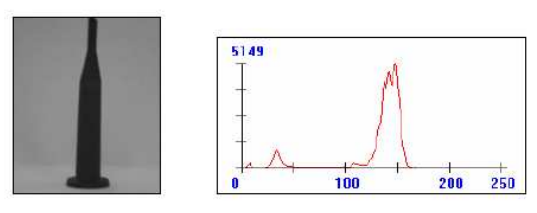
\includegraphics[scale= 0.40]{images/L8_Clus_thr1D.png}}\\
\item Clustering in 2D, color image $\rightarrow$ color thresholding
\centering{
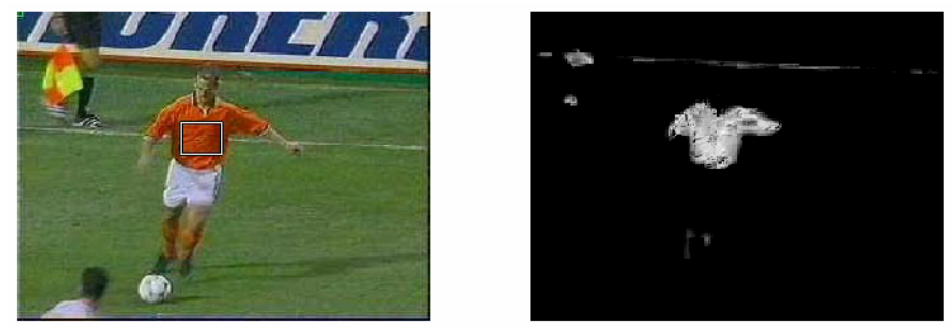
\includegraphics[scale=0.25]{images/L8_Clus_Imthr1.png}\
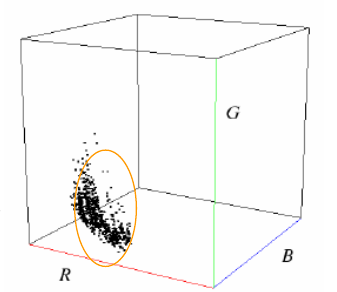
\includegraphics[scale=0.25]{images/L8_Clus_Imthr2.png}}
\end{itemize}
\end{block}
\end{frame}

\begin{frame}
\frametitle{Clustering Techniques}
\begin{block}{Thresholding}
\scriptsize{
\begin{itemize}
\item Fixed or Global threshold: Threshold value is fixed through the image \\
\centering{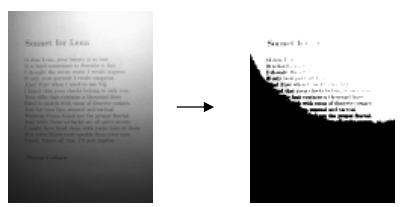
\includegraphics[scale=0.4]{images/L8_ex_Gth.png}}\\
\item Local or Adaptive threshold: Two or more threshold is used through the image\\
\item Local or Adaptive threshold: Local threshold for small patches, Patch size ($7 \times 7$), $P_{T_{1}} = \mu$, $P_{T_{2}} = \mu -7$, $P_{T_{3}} = \mu-10$
\end{itemize}

}
\centering{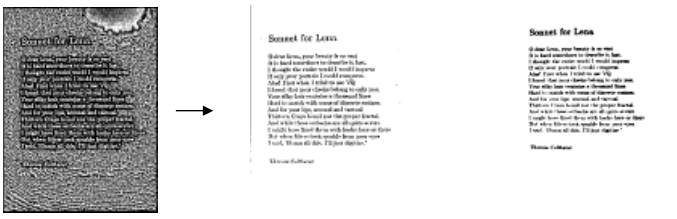
\includegraphics[scale=0.4]{images/L8_ex_Ath.png}}
\end{block}
\end{frame}


\begin{frame}
\frametitle{Clustering Techniques}
\begin{block}{Optimal Thresholding}
\begin{itemize}
\footnotesize{
\item Isodata, Peak and valley, Otsu, p-tile,...
\item \textbf{ISODATA} (Iterative Self-Organising Data Analysis Technique Algorithm):} \\
\begin{itemize}
\scriptsize{
\item $T_{i} = T_{0}$, median, maximum gray level, ...
\item Segmenting the histogram into two parts
\item Computing the mean value associated to each part ($\mu_{1}, \mu_{2}$)
\item New threshold, $T_{i+1} = (\mu_{1}+ \mu_{2})/2$
\item Repeat until convergence, $T_{i} = T_{i-1}$

}
\end{itemize}

\end{itemize}

\end{block}
\end{frame}
%-------------
\section{Edge Based}

%---------------
%-----------
\end{document}

%\begin{itemize}
%\item Also use neighborhood but do not use coefficients 
%\begin{itemize}
%\item median filter for noise reduction
%\end{itemize} 
%\end{itemize}
